

%-------------------------------------------------------------------------------
% Dokumenten Klasse
\documentclass[
	final,
	a4paper,
	oneside,
	parskip=full,
	headings=standardclasses,
	headings=big,
	pointednumbers
]{scrartcl}

%-------------------------------------------------------------------------------
% Packete nutzen
\usepackage[T1]{fontenc}
\usepackage[utf8]{inputenc}
\usepackage[left=20mm,right=25mm,top=20mm,bottom=25mm]{geometry}
\usepackage{amsmath}
\usepackage{amssymb}
\usepackage{mathtools}
\usepackage{mathtools}

%-------------------------------------------------------------------------------
% xcolor
\usepackage[svgnames]{xcolor}

%-------------------------------------------------------------------------------
% tabularx
\usepackage{tabularx}
\usepackage{ltablex}
\usepackage{makecell}

%-------------------------------------------------------------------------------
% TikZ
\usepackage{tikz}
\usetikzlibrary{positioning, arrows, decorations, calc, fit}

%-------------------------------------------------------------------------------
% Listings
\usepackage{listings}
\newcommand{\listingMatlab}[2][]{
	\lstset{
		language=Matlab,
		breaklines=true,
		numbers=left,
		numberstyle=\tiny,
		numbersep=5pt,
		captionpos=b,
		basicstyle=\footnotesize\ttfamily,
		stringstyle=\color{magenta},
		identifierstyle=\color{black},
		keywordstyle=\color{blue}, 
		commentstyle=\color{DarkGreen}
	}
	\lstinputlisting[caption={\texttt{\detokenize{#2}}},#1]{#2}
}
\lstnewenvironment{algorithm}[1][] %defines the algorithm listing environment
{
    \lstset{ %this is the stype
        mathescape=true,
        frame=tB,
        numbers=left, 
        numberstyle=\tiny,
        basicstyle=\scriptsize, 
        keywordstyle=\color{black}\bfseries,
        keywords={,input, output, return, datatype, function, in, if, else, foreach, while, begin, end, } 
        numbers=left,
        xleftmargin=.04\textwidth
    }
}
{}

%-------------------------------------------------------------------------------
% 
\newcommand{\f}[2]{\frac{#1}{#2}}
\newcommand{\fs}[2]{{\tfrac{#1}{#2}}}

% kl = ()
\newcommand{\kl}[1]{{\left( #1 \right)}}

% kq = {}
\newcommand{\kq}[1]{{\left\{ #1 \right\}}}

% ks = []
\newcommand{\ks}[1]{{\left[ #1 \right]}}

% 
\newcommand{\abs}[1]{{\vert #1 \vert}}

\newcommand\addvmargin[1]{
  \node[fit=(current bounding box),inner ysep=#1,inner xsep=0]{};
}

\def\tiktop{%
    \def\xlines{15}
    \def\ylines{11}
    \def\raster{5mm}

    \coordinate (p1) at (0*\raster,5*\raster);
    \coordinate (p2) at (1*\raster,3*\raster);
    \coordinate (p3) at (2*\raster,1*\raster);
    \coordinate (p4) at (3*\raster,9*\raster);
    \coordinate (p5) at (4*\raster,6*\raster);
    \coordinate (p6) at (5*\raster,0*\raster);
    \coordinate (p7) at (6*\raster,11*\raster);
    \coordinate (p8) at (7*\raster,5*\raster);
    \coordinate (p9) at (7*\raster,7*\raster);
    \coordinate (p10) at (8*\raster,9*\raster);
    \coordinate (p11) at (9*\raster,6*\raster);
    \coordinate (p12) at (10*\raster,1*\raster);
    \coordinate (p13) at (11*\raster,10*\raster);
    \coordinate (p14) at (12*\raster,5*\raster);
    \coordinate (p15) at (13*\raster,0*\raster);
    \coordinate (p16) at (14*\raster,8*\raster);
    \coordinate (p17) at (15*\raster,5*\raster);
    % draw vertical lines
    \foreach \x in {0,...,\xlines}
    {
        \draw[lightgray] (\x * \raster, 0mm) -- (\x * \raster, \ylines * \raster);
    }

    % draw horizontal lines
    \foreach \y in {0,...,\ylines}
    {
        \draw[lightgray] (0mm, \y * \raster) -- (\xlines * \raster, \y * \raster);
    }

    % border
    \draw[black] (0mm, 0mm) -- (\xlines * \raster, 0mm);
    \draw[black] (0mm, 0mm) -- (0mm, \ylines * \raster);
    \draw[black] (\xlines * \raster, 0mm) -- (\xlines * \raster, \ylines * \raster);
    \draw[black] (0mm, \ylines * \raster) -- (\xlines * \raster, \ylines * \raster);
}

\def\Lupper{\mathcal{L}_{\mathrm{upper}}}
\def\Llower{\mathcal{L}_{\mathrm{lower}}}

\def\pich{6cm}
\def\picb{8cm}

\begin{document}

    \begin{tabularx}{\textwidth}{rl}
        % --- LINE 1 --------------------------------------------------------
        \noindent\parbox[c][\pich]{\picb}{
        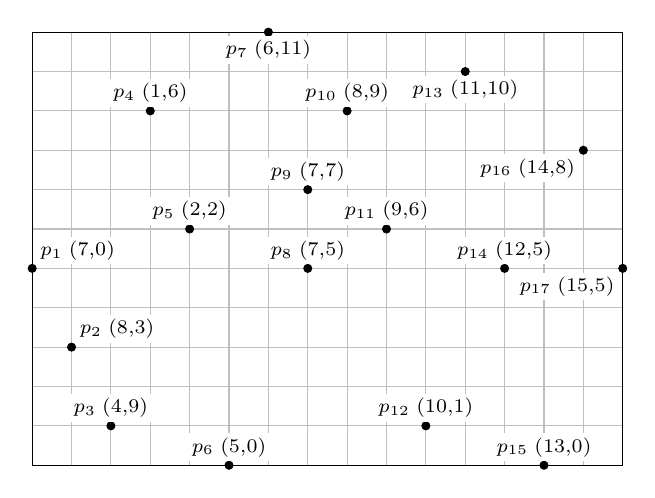
\begin{tikzpicture}[baseline=0]
            \tiktop
            
            \foreach \point/\a/\b/\i/\align in {
                p1/7/0/1/above right,
                p2/8/3/2/above right,
                p3/4/9/3/above,
                p4/1/6/4/above,
                p5/2/2/5/above,
                p6/5/0/6/above,
                p7/6/11/7/below,
                p8/7/5/8/above,
                p9/7/7/9/above,
                p10/8/9/10/above,
                p11/9/6/11/above,
                p12/10/1/12/above,
                p13/11/10/13/below,
                p14/12/5/14/above,
                p15/13/0/15/above,
                p16/14/8/16/below left,
                p17/15/5/17/below left}{

                \draw[black,fill=black]
                    let \p1 = (\point)
                    in (\x1, \y1) circle (0.5mm);
                \path
                    let \p1 = (\point)
                    in
                        node[\align, fill=white, inner sep=1.5, outer sep=1.5] at (\x1, \y1) {$\scriptstyle p_{\i} \; \left( \a, \b \right) $};
            }
        \end{tikzpicture}} &
        {$\!\begin{aligned}[t]
            
        \end{aligned}
        $} \\
        % --- LINE 2 --------------------------------------------------------
        \noindent\parbox[c][\pich]{\picb}{
        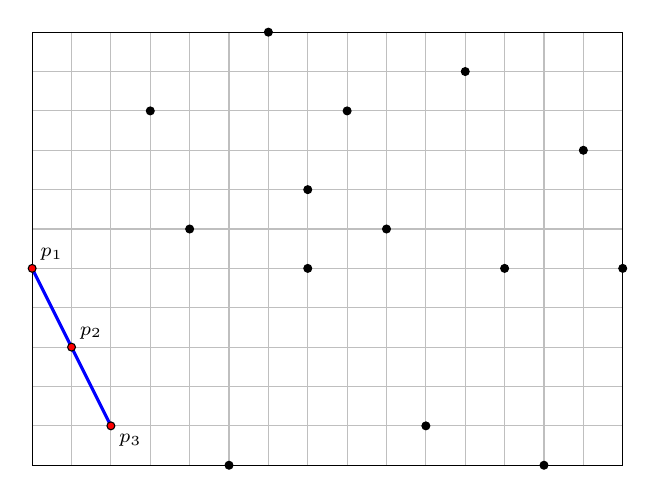
\begin{tikzpicture}[baseline=0]
            \tiktop
            
            \draw[blue, line width=0.4mm]
                (p1) -- (p2) -- (p3);

            \foreach \point/\a/\b/\i/\align/\co in {
                p1/7/0/1/above right/red,
                p2/8/3/2/above right/red,
                p3/4/9/3/above/red,
                p4/1/6/4/above/black,
                p5/2/2/5/above/black,
                p6/5/0/6/above/black,
                p7/6/11/7/below/black,
                p8/7/5/8/above/black,
                p9/7/7/9/above/black,
                p10/8/9/10/above/black,
                p11/9/6/11/above/black,
                p12/10/1/12/above/black,
                p13/11/10/13/below/black,
                p14/12/5/14/above/black,
                p15/13/0/15/above/black,
                p16/14/8/16/below left/black,
                p17/15/5/17/below left/black}{

                \draw[black,fill=\co]
                    let \p1 = (\point)
                    in (\x1, \y1) circle (0.5mm);
            }
            \foreach \point/\a/\b/\i/\align in {
                p1/7/0/1/above right,
                p2/8/3/2/above right,
                p3/4/9/3/below right}{

                \path
                    let \p1 = (\point)
                    in
                        node[\align, fill=white, inner sep=1.5, outer sep=1.5] at (\x1, \y1) {$\scriptstyle p_{\i} $};
            }
        \end{tikzpicture}} &
        \makecell[l]{$\!\begin{aligned}
            & \Lupper = \kq{p_1,p_2} \\
            & \text{Append } p_3 \text{ to } \Lupper \\
            & \abs{\Lupper} > 2 \text{: contains more than two points} \rightarrow \text{true} \\
            & \text{last three points in } \Lupper \text{ do not make right turn} \rightarrow \text{true} \\
            & \text{Delete middle point } p_2
        \end{aligned}$} \\

        % --- LINE 3 --------------------------------------------------------
        \noindent\parbox[c][\pich]{\picb}{
        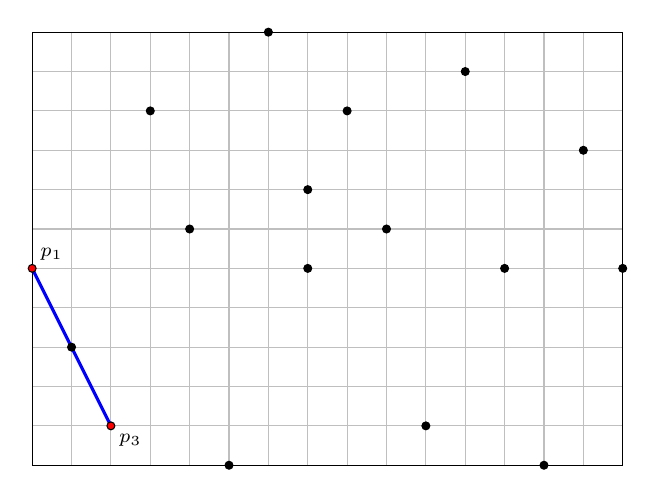
\begin{tikzpicture}[baseline=0]
            \tiktop
            
            \draw[blue, line width=0.4mm]
                (p1) -- (p3);

            \foreach \point/\a/\b/\i/\align/\co in {
                p1/7/0/1/above right/red,
                p2/8/3/2/above right/black,
                p3/4/9/3/above/red,
                p4/1/6/4/above/black,
                p5/2/2/5/above/black,
                p6/5/0/6/above/black,
                p7/6/11/7/below/black,
                p8/7/5/8/above/black,
                p9/7/7/9/above/black,
                p10/8/9/10/above/black,
                p11/9/6/11/above/black,
                p12/10/1/12/above/black,
                p13/11/10/13/below/black,
                p14/12/5/14/above/black,
                p15/13/0/15/above/black,
                p16/14/8/16/below left/black,
                p17/15/5/17/below left/black}{

                \draw[black,fill=\co]
                    let \p1 = (\point)
                    in (\x1, \y1) circle (0.5mm);
            }
            \foreach \point/\a/\b/\i/\align in {
                p1/7/0/1/above right,
                p3/4/9/3/below right}{

                \path
                    let \p1 = (\point)
                    in
                        node[\align, fill=white, inner sep=1.5, outer sep=1.5] at (\x1, \y1) {$\scriptstyle p_{\i} $};
            }
        \end{tikzpicture}} &
        \makecell[l]{$\!\begin{aligned}
            & \Lupper = \kq{p_1,p_3} \\
            & \abs{\Lupper} > 2 \text{: contains more than two points} \rightarrow \text{false}
        \end{aligned}$} \\
        % --- LINE 4 --------------------------------------------------------
        \noindent\parbox[c][\pich]{\picb}{
        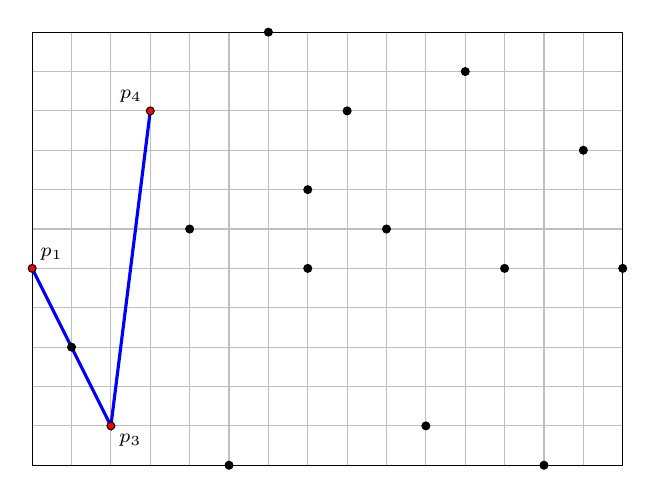
\begin{tikzpicture}[baseline=0]
            \tiktop
            
            \draw[blue, line width=0.4mm]
                (p1) -- (p3) -- (p4);

            \foreach \point/\a/\b/\i/\align/\co in {
                p1/7/0/1/above right/red,
                p2/8/3/2/above right/black,
                p3/4/9/3/above/red,
                p4/1/6/4/above/red,
                p5/2/2/5/above/black,
                p6/5/0/6/above/black,
                p7/6/11/7/below/black,
                p8/7/5/8/above/black,
                p9/7/7/9/above/black,
                p10/8/9/10/above/black,
                p11/9/6/11/above/black,
                p12/10/1/12/above/black,
                p13/11/10/13/below/black,
                p14/12/5/14/above/black,
                p15/13/0/15/above/black,
                p16/14/8/16/below left/black,
                p17/15/5/17/below left/black}{

                \draw[black,fill=\co]
                    let \p1 = (\point)
                    in (\x1, \y1) circle (0.5mm);
            }
            \foreach \point/\a/\b/\i/\align in {
                p1/7/0/1/above right,
                p3/4/9/3/below right,
                p4/1/6/4/above left}{

                \path
                    let \p1 = (\point)
                    in
                        node[\align, fill=white, inner sep=1.5, outer sep=1.5] at (\x1, \y1) {$\scriptstyle p_{\i} $};
            }
        \end{tikzpicture}} &
        \makecell[l]{$\!\begin{aligned}
            & \Lupper = \kq{p_1,p_3} \\
            & \abs{\Lupper} > 2 \text{: contains more than two points} \rightarrow \text{false} \\
            & \text{Append } p_4 \text{ to } \Lupper \\
            & \abs{\Lupper} > 2 \text{: contains more than two points} \rightarrow \text{true} \\
            & \text{last three points in } \Lupper \text{ do not make right turn} \rightarrow \text{true} \\
            & \text{Delete middle point } p_3
        \end{aligned}$} \\
        % --- LINE 5 --------------------------------------------------------
        \noindent\parbox[c][\pich]{\picb}{
        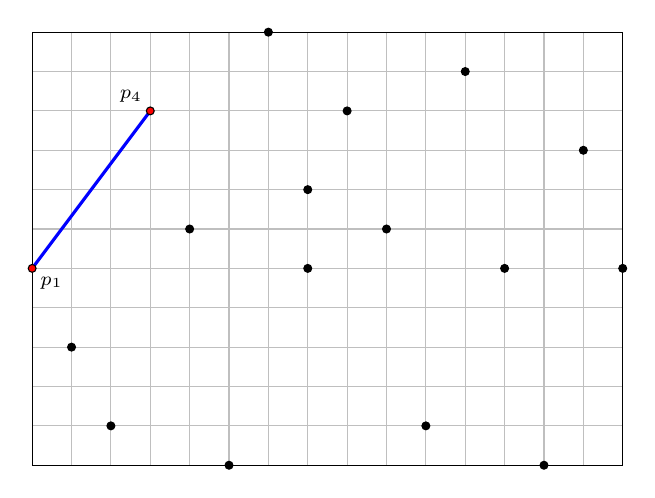
\begin{tikzpicture}[baseline=0]
            \tiktop
            
            \draw[blue, line width=0.4mm]
                (p1) -- (p4);

            \foreach \point/\a/\b/\i/\align/\co in {
                p1/7/0/1/above right/red,
                p2/8/3/2/above right/black,
                p3/4/9/3/above/black,
                p4/1/6/4/above/red,
                p5/2/2/5/above/black,
                p6/5/0/6/above/black,
                p7/6/11/7/below/black,
                p8/7/5/8/above/black,
                p9/7/7/9/above/black,
                p10/8/9/10/above/black,
                p11/9/6/11/above/black,
                p12/10/1/12/above/black,
                p13/11/10/13/below/black,
                p14/12/5/14/above/black,
                p15/13/0/15/above/black,
                p16/14/8/16/below left/black,
                p17/15/5/17/below left/black}{

                \draw[black,fill=\co]
                    let \p1 = (\point)
                    in (\x1, \y1) circle (0.5mm);
            }
            \foreach \point/\a/\b/\i/\align/\co in {
                p1/7/0/1/below right/black,
                p4/1/6/4/above left/black}{

                \path
                    let \p1 = (\point)
                    in
                        node[\align, fill=white, inner sep=1.5, outer sep=1.5] at (\x1, \y1) {$\scriptstyle p_{\i} $};
            }
        \end{tikzpicture}} &
        \makecell[l]{$\!\begin{aligned}
            & \Lupper = \kq{p_1,p_4} \\
            & \abs{\Lupper} > 2 \text{: contains more than two points} \rightarrow \text{false} \\
        \end{aligned}$} \\
        % --- LINE 6 --------------------------------------------------------
        \noindent\parbox[c][\pich]{\picb}{
        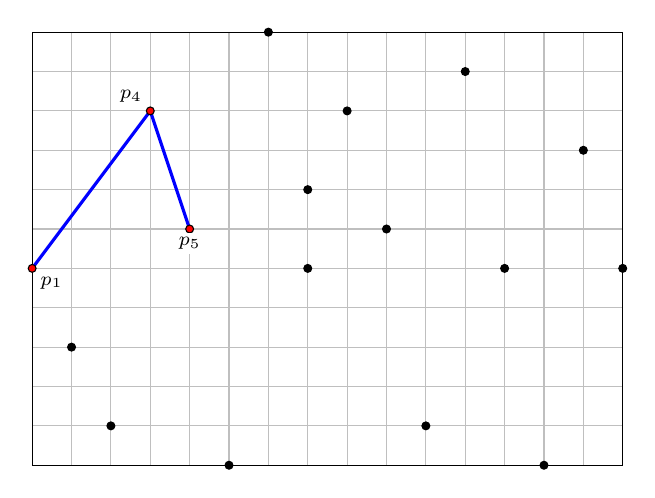
\begin{tikzpicture}[baseline=0]
            \tiktop
            
            \draw[blue, line width=0.4mm]
                (p1) -- (p4) -- (p5);

            \foreach \point/\a/\b/\i/\align/\co in {
                p1/7/0/1/above right/red,
                p2/8/3/2/above right/black,
                p3/4/9/3/above/black,
                p4/1/6/4/above/red,
                p5/2/2/5/above/red,
                p6/5/0/6/above/black,
                p7/6/11/7/below/black,
                p8/7/5/8/above/black,
                p9/7/7/9/above/black,
                p10/8/9/10/above/black,
                p11/9/6/11/above/black,
                p12/10/1/12/above/black,
                p13/11/10/13/below/black,
                p14/12/5/14/above/black,
                p15/13/0/15/above/black,
                p16/14/8/16/below left/black,
                p17/15/5/17/below left/black}{

                \draw[black,fill=\co]
                    let \p1 = (\point)
                    in (\x1, \y1) circle (0.5mm);
            }
            \foreach \point/\a/\b/\i/\align/\co in {
                p1/7/0/1/below right/black,
                p4/1/6/4/above left/black,
                p5/2/2/5/below/black}{

                \path
                    let \p1 = (\point)
                    in
                        node[\align, fill=white, inner sep=1.5, outer sep=1.5] at (\x1, \y1) {$\scriptstyle p_{\i} $};
            }
        \end{tikzpicture}} &
        \makecell[l]{$\!\begin{aligned}
            & \Lupper = \kq{p_1,p_4} \\
            & \text{Append } p_5 \text{ to } \Lupper \\
            & \abs{\Lupper} > 2 \text{: contains more than two points} \rightarrow \text{true} \\
            & \text{last three points in } \Lupper \text{ do not make right turn} \rightarrow \text{false}
        \end{aligned}$} \\
        % --- LINE 7 --------------------------------------------------------
        \noindent\parbox[c][\pich]{\picb}{
        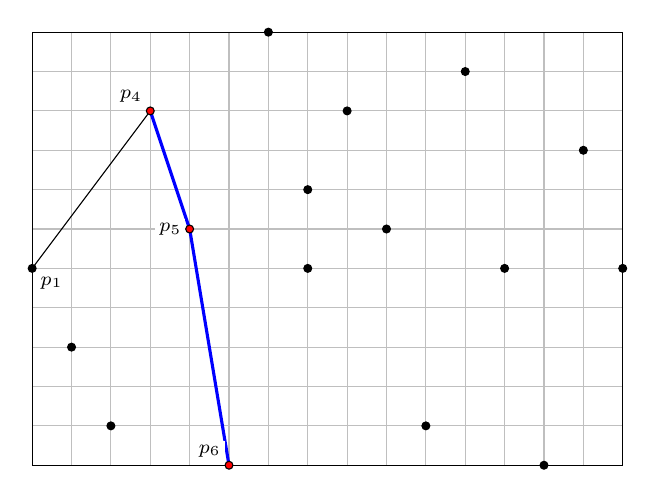
\begin{tikzpicture}[baseline=0]
            \tiktop
            
            \draw[black]
                (p1) -- (p4);
            \draw[blue, line width=0.4mm]
                (p4) -- (p5) -- (p6);

            \foreach \point/\a/\b/\i/\align/\co in {
                p1/7/0/1/above right/black,
                p2/8/3/2/above right/black,
                p3/4/9/3/above/black,
                p4/1/6/4/above/red,
                p5/2/2/5/above/red,
                p6/5/0/6/above/red,
                p7/6/11/7/below/black,
                p8/7/5/8/above/black,
                p9/7/7/9/above/black,
                p10/8/9/10/above/black,
                p11/9/6/11/above/black,
                p12/10/1/12/above/black,
                p13/11/10/13/below/black,
                p14/12/5/14/above/black,
                p15/13/0/15/above/black,
                p16/14/8/16/below left/black,
                p17/15/5/17/below left/black}{

                \draw[black,fill=\co]
                    let \p1 = (\point)
                    in (\x1, \y1) circle (0.5mm);
            }
            \foreach \point/\a/\b/\i/\align/\co in {
                p1/7/0/1/below right/black,
                p4/1/6/4/above left/black,
                p5/2/2/5/left/black,
                p6/5/0/6/above left/red}{

                \path
                    let \p1 = (\point)
                    in
                        node[\align, fill=white, inner sep=1.5, outer sep=1.5] at (\x1, \y1) {$\scriptstyle p_{\i} $};
            }
        \end{tikzpicture}} &
        \makecell[l]{$\!\begin{aligned}
            & \Lupper = \kq{p_1,p_4, p_5} \\
            & \text{Append } p_6 \text{ to } \Lupper \\
            & \abs{\Lupper} > 2 \text{: contains more than two points} \rightarrow \text{true} \\
            & \text{last three points in } \Lupper \text{ do not make right turn} \rightarrow \text{false}
        \end{aligned}$} \\
        % --- LINE 8 --------------------------------------------------------
        \noindent\parbox[c][\pich]{\picb}{
        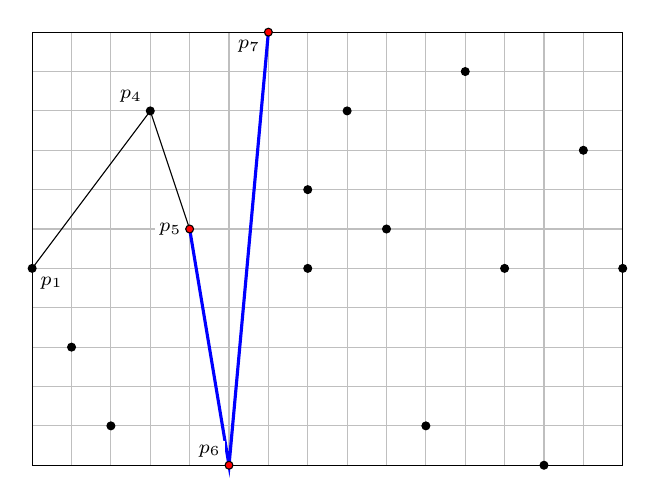
\begin{tikzpicture}[baseline=0]
            \tiktop
            
            \draw[black]
                (p1) -- (p4) -- (p5);
            \draw[blue, line width=0.4mm]
                (p5) -- (p6) -- (p7);

            \foreach \point/\a/\b/\i/\align/\co in {
                p1/7/0/1/above right/black,
                p2/8/3/2/above right/black,
                p3/4/9/3/above/black,
                p4/1/6/4/above/black,
                p5/2/2/5/above/red,
                p6/5/0/6/above/red,
                p7/6/11/7/below/red,
                p8/7/5/8/above/black,
                p9/7/7/9/above/black,
                p10/8/9/10/above/black,
                p11/9/6/11/above/black,
                p12/10/1/12/above/black,
                p13/11/10/13/below/black,
                p14/12/5/14/above/black,
                p15/13/0/15/above/black,
                p16/14/8/16/below left/black,
                p17/15/5/17/below left/black}{

                \draw[black,fill=\co]
                    let \p1 = (\point)
                    in (\x1, \y1) circle (0.5mm);
            }
            \foreach \point/\a/\b/\i/\align/\co in {
                p1/7/0/1/below right/black,
                p4/1/6/4/above left/black,
                p5/2/2/5/left/black,
                p6/5/0/6/above left/red,
                p7/6/11/7/below left/black}{

                \path
                    let \p1 = (\point)
                    in
                        node[\align, fill=white, inner sep=1.5, outer sep=1.5] at (\x1, \y1) {$\scriptstyle p_{\i} $};
            }
        \end{tikzpicture}} &
        \makecell[l]{$\!\begin{aligned}
            & \Lupper = \kq{p_1,p_4, p_5, p_6} \\
            & \text{Append } p_7 \text{ to } \Lupper \\
            & \abs{\Lupper} > 2 \text{: contains more than two points} \rightarrow \text{true} \\
            & \text{last three points in } \Lupper \text{ do not make right turn} \rightarrow \text{true} \\
            & \text{Delete middle point } p_6
        \end{aligned}$} \\
        % --- LINE 9 --------------------------------------------------------
        \noindent\parbox[c][\pich]{\picb}{
        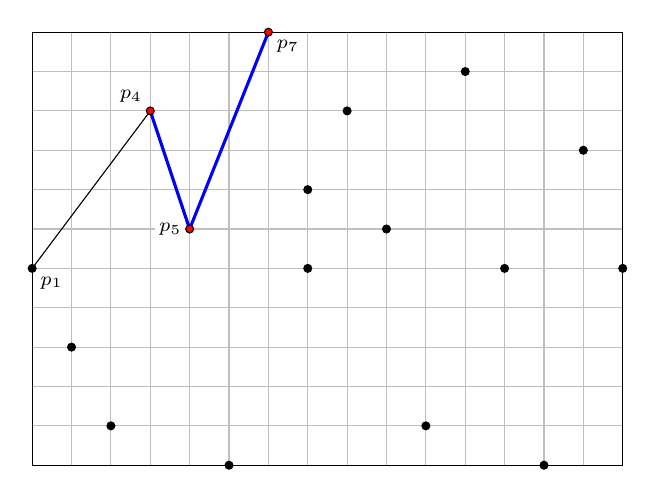
\begin{tikzpicture}[baseline=0]
            \tiktop
            
            \draw[black]
                (p1) -- (p4);
            \draw[blue, line width=0.4mm]
                (p4) -- (p5) -- (p7);

            \foreach \point/\a/\b/\i/\align/\co in {
                p1/7/0/1/above right/black,
                p2/8/3/2/above right/black,
                p3/4/9/3/above/black,
                p4/1/6/4/above/red,
                p5/2/2/5/above/red,
                p6/5/0/6/above/black,
                p7/6/11/7/below/red,
                p8/7/5/8/above/black,
                p9/7/7/9/above/black,
                p10/8/9/10/above/black,
                p11/9/6/11/above/black,
                p12/10/1/12/above/black,
                p13/11/10/13/below/black,
                p14/12/5/14/above/black,
                p15/13/0/15/above/black,
                p16/14/8/16/below left/black,
                p17/15/5/17/below left/black}{

                \draw[black,fill=\co]
                    let \p1 = (\point)
                    in (\x1, \y1) circle (0.5mm);
            }
            \foreach \point/\a/\b/\i/\align/\co in {
                p1/7/0/1/below right/black,
                p4/1/6/4/above left/black,
                p5/2/2/5/left/black,
                p7/6/11/7/below right/black}{

                \path
                    let \p1 = (\point)
                    in
                        node[\align, fill=white, inner sep=1.5, outer sep=1.5] at (\x1, \y1) {$\scriptstyle p_{\i} $};
            }
        \end{tikzpicture}} &
        \makecell[l]{$\!\begin{aligned}
            & \Lupper = \kq{p_1,p_4, p_5, p_7} \\
            & \abs{\Lupper} > 2 \text{: contains more than two points} \rightarrow \text{true} \\
            & \text{last three points in } \Lupper \text{ do not make right turn} \rightarrow \text{true} \\
            & \text{Delete middle point } p_5
        \end{aligned}$} \\
        % --- LINE 10 --------------------------------------------------------
        \noindent\parbox[c][\pich]{\picb}{
        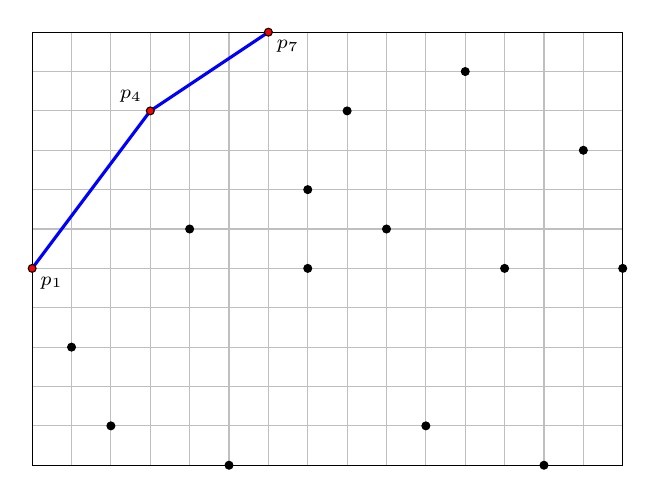
\begin{tikzpicture}[baseline=0]
            \tiktop
            
            \draw[blue, line width=0.4mm]
                (p1) -- (p4) -- (p7);

            \foreach \point/\a/\b/\i/\align/\co in {
                p1/7/0/1/above right/red,
                p2/8/3/2/above right/black,
                p3/4/9/3/above/black,
                p4/1/6/4/above/red,
                p5/2/2/5/above/black,
                p6/5/0/6/above/black,
                p7/6/11/7/below/red,
                p8/7/5/8/above/black,
                p9/7/7/9/above/black,
                p10/8/9/10/above/black,
                p11/9/6/11/above/black,
                p12/10/1/12/above/black,
                p13/11/10/13/below/black,
                p14/12/5/14/above/black,
                p15/13/0/15/above/black,
                p16/14/8/16/below left/black,
                p17/15/5/17/below left/black}{

                \draw[black,fill=\co]
                    let \p1 = (\point)
                    in (\x1, \y1) circle (0.5mm);
            }
            \foreach \point/\a/\b/\i/\align/\co in {
                p1/7/0/1/below right/black,
                p4/1/6/4/above left/black,
                p7/6/11/7/below right/black}{

                \path
                    let \p1 = (\point)
                    in
                        node[\align, fill=white, inner sep=1.5, outer sep=1.5] at (\x1, \y1) {$\scriptstyle p_{\i} $};
            }
        \end{tikzpicture}} &
        \makecell[l]{$\!\begin{aligned}
            & \Lupper = \kq{p_1,p_4, p_7}
        \end{aligned}$} \\
        % --- LINE 11 --------------------------------------------------------
        \noindent\parbox[c][\pich]{\picb}{
        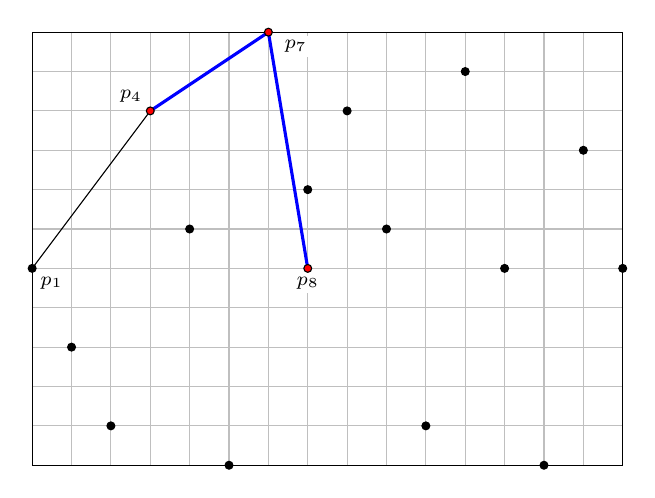
\begin{tikzpicture}[baseline=0]
            \tiktop
            
            \draw[black]
                (p1) -- (p4);
            \draw[blue, line width=0.4mm]
                (p4) -- (p7) -- (p8);

            \foreach \point/\a/\b/\i/\align/\co in {
                p1/7/0/1/above right/black,
                p2/8/3/2/above right/black,
                p3/4/9/3/above/black,
                p4/1/6/4/above/red,
                p5/2/2/5/above/black,
                p6/5/0/6/above/black,
                p7/6/11/7/below/red,
                p8/7/5/8/above/red,
                p9/7/7/9/above/black,
                p10/8/9/10/above/black,
                p11/9/6/11/above/black,
                p12/10/1/12/above/black,
                p13/11/10/13/below/black,
                p14/12/5/14/above/black,
                p15/13/0/15/above/black,
                p16/14/8/16/below left/black,
                p17/15/5/17/below left/black}{

                \draw[black,fill=\co]
                    let \p1 = (\point)
                    in (\x1, \y1) circle (0.5mm);
            }
            \foreach \point/\a/\b/\i/\align/\co in {
                p1/7/0/1/below right/black,
                p4/1/6/4/above left/black,
                p8/7/5/8/below/red}{

                \path
                    let \p1 = (\point)
                    in
                        node[\align, fill=white, inner sep=1.5, outer sep=1.5] at (\x1, \y1) {$\scriptstyle p_{\i} $};
            }
            \foreach \point/\a/\b/\i/\align/\co in {
                p7/6/11/7/below right/black}{

                \path
                    let \p1 = (\point)
                    in
                        node[\align, xshift=1mm, fill=white, inner sep=1.5, outer sep=1.5] at (\x1, \y1) {$\scriptstyle p_{\i} $};
            }
        \end{tikzpicture}} &
        \makecell[l]{$\!\begin{aligned}
            & \Lupper = \kq{p_1,p_4, p_7} \\
            & \text{Append } p_8 \text{ to } \Lupper \\
            & \abs{\Lupper} > 2 \text{: contains more than two points} \rightarrow \text{true} \\
            & \text{last three points in } \Lupper \text{ do not make right turn} \rightarrow \text{false}
        \end{aligned}$} \\
        % --- LINE 12 --------------------------------------------------------
        \noindent\parbox[c][\pich]{\picb}{
        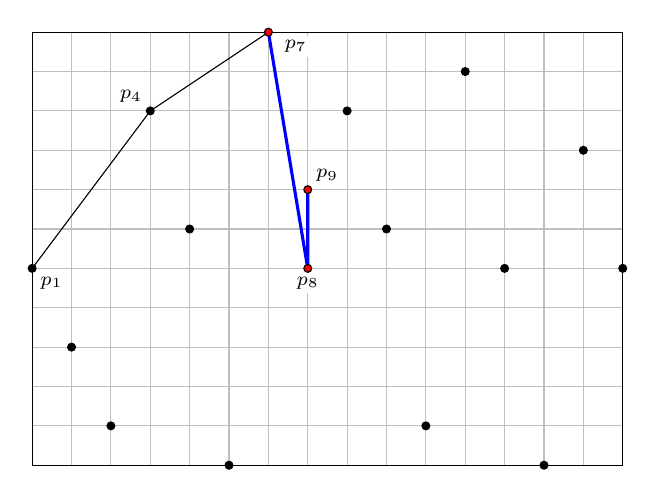
\begin{tikzpicture}[baseline=0]
            \tiktop
            
            \draw[black]
                (p1) -- (p4) -- (p7);
            \draw[blue, line width=0.4mm]
                (p7) -- (p8) -- (p9);

            \foreach \point/\a/\b/\i/\align/\co in {
                p1/7/0/1/above right/black,
                p2/8/3/2/above right/black,
                p3/4/9/3/above/black,
                p4/1/6/4/above/black,
                p5/2/2/5/above/black,
                p6/5/0/6/above/black,
                p7/6/11/7/below/red,
                p8/7/5/8/above/red,
                p9/7/7/9/above/red,
                p10/8/9/10/above/black,
                p11/9/6/11/above/black,
                p12/10/1/12/above/black,
                p13/11/10/13/below/black,
                p14/12/5/14/above/black,
                p15/13/0/15/above/black,
                p16/14/8/16/below left/black,
                p17/15/5/17/below left/black}{

                \draw[black,fill=\co]
                    let \p1 = (\point)
                    in (\x1, \y1) circle (0.5mm);
            }
            \foreach \point/\a/\b/\i/\align/\co in {
                p1/7/0/1/below right/black,
                p4/1/6/4/above left/black,
                p8/7/5/8/below/red,
                p9/7/7/9/above right/red}{

                \path
                    let \p1 = (\point)
                    in
                        node[\align, fill=white, inner sep=1.5, outer sep=1.5] at (\x1, \y1) {$\scriptstyle p_{\i} $};
            }
            \foreach \point/\a/\b/\i/\align/\co in {
                p7/6/11/7/below right/black}{

                \path
                    let \p1 = (\point)
                    in
                        node[\align, xshift=1mm, fill=white, inner sep=1.5, outer sep=1.5] at (\x1, \y1) {$\scriptstyle p_{\i} $};
            }
        \end{tikzpicture}} &
        \makecell[l]{$\!\begin{aligned}
            & \Lupper = \kq{p_1,p_4, p_7, p_8} \\
            & \text{Append } p_9 \text{ to } \Lupper \\
            & \abs{\Lupper} > 2 \text{: contains more than two points} \rightarrow \text{true} \\
            & \text{last three points in } \Lupper \text{ do not make right turn} \rightarrow \text{true} \\
            & \text{Delete middle point } p_8
        \end{aligned}$} \\
        % --- LINE 13 --------------------------------------------------------
        \noindent\parbox[c][\pich]{\picb}{
        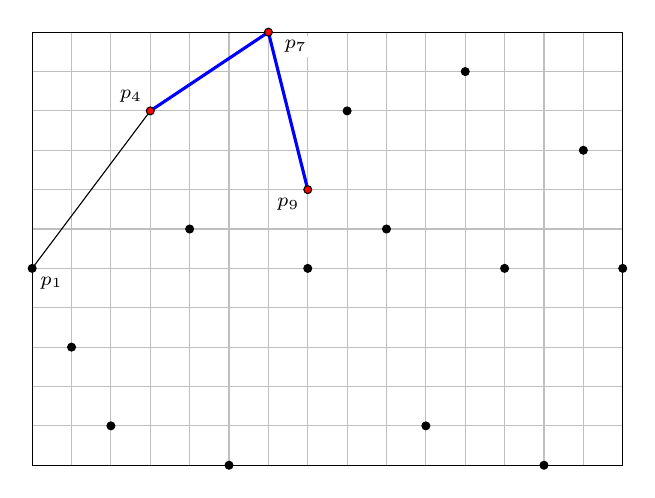
\begin{tikzpicture}[baseline=0]
            \tiktop
            
            \draw[black]
                (p1) -- (p4);
            \draw[blue, line width=0.4mm]
                (p4) -- (p7) -- (p9);

            \foreach \point/\a/\b/\i/\align/\co in {
                p1/7/0/1/above right/black,
                p2/8/3/2/above right/black,
                p3/4/9/3/above/black,
                p4/1/6/4/above/red,
                p5/2/2/5/above/black,
                p6/5/0/6/above/black,
                p7/6/11/7/below/red,
                p8/7/5/8/above/black,
                p9/7/7/9/above/red,
                p10/8/9/10/above/black,
                p11/9/6/11/above/black,
                p12/10/1/12/above/black,
                p13/11/10/13/below/black,
                p14/12/5/14/above/black,
                p15/13/0/15/above/black,
                p16/14/8/16/below left/black,
                p17/15/5/17/below left/black}{

                \draw[black,fill=\co]
                    let \p1 = (\point)
                    in (\x1, \y1) circle (0.5mm);
            }
            \foreach \point/\a/\b/\i/\align/\co in {
                p1/7/0/1/below right/black,
                p4/1/6/4/above left/black,
                p9/7/7/9/below left/red}{

                \path
                    let \p1 = (\point)
                    in
                        node[\align, fill=white, inner sep=1.5, outer sep=1.5] at (\x1, \y1) {$\scriptstyle p_{\i} $};
            }
            \foreach \point/\a/\b/\i/\align/\co in {
                p7/6/11/7/below right/black}{

                \path
                    let \p1 = (\point)
                    in
                        node[\align, xshift=1mm, fill=white, inner sep=1.5, outer sep=1.5] at (\x1, \y1) {$\scriptstyle p_{\i} $};
            }
        \end{tikzpicture}} &
        \makecell[l]{$\!\begin{aligned}
            & \Lupper = \kq{p_1,p_4, p_7, p_8} \\
            & \abs{\Lupper} > 2 \text{: contains more than two points} \rightarrow \text{true} \\
            & \text{last three points in } \Lupper \text{ do not make right turn} \rightarrow \text{false}
        \end{aligned}$} \\
        % --- LINE 14 --------------------------------------------------------
        \noindent\parbox[c][\pich]{\picb}{
        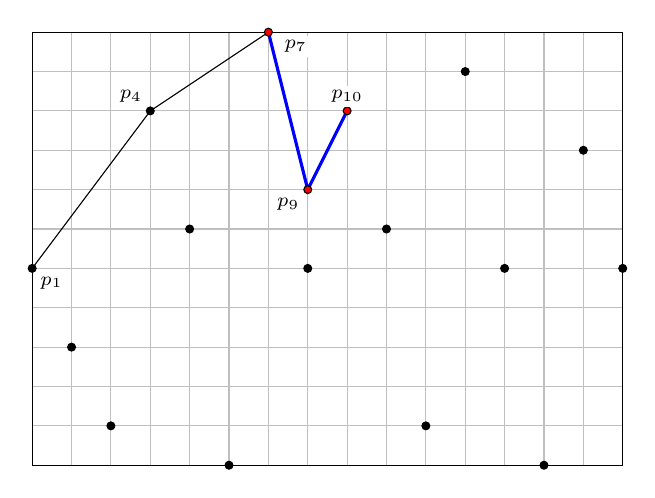
\begin{tikzpicture}[baseline=0]
            \tiktop
            
            \draw[black]
                (p1) -- (p4) -- (p7);
            \draw[blue, line width=0.4mm]
                (p7) -- (p9) -- (p10);

            \foreach \point/\a/\b/\i/\align/\co in {
                p1/7/0/1/above right/black,
                p2/8/3/2/above right/black,
                p3/4/9/3/above/black,
                p4/1/6/4/above/black,
                p5/2/2/5/above/black,
                p6/5/0/6/above/black,
                p7/6/11/7/below/red,
                p8/7/5/8/above/black,
                p9/7/7/9/above/red,
                p10/8/9/10/above/red,
                p11/9/6/11/above/black,
                p12/10/1/12/above/black,
                p13/11/10/13/below/black,
                p14/12/5/14/above/black,
                p15/13/0/15/above/black,
                p16/14/8/16/below left/black,
                p17/15/5/17/below left/black}{

                \draw[black,fill=\co]
                    let \p1 = (\point)
                    in (\x1, \y1) circle (0.5mm);
            }
            \foreach \point/\a/\b/\i/\align/\co in {
                p1/7/0/1/below right/black,
                p4/1/6/4/above left/black,
                p9/7/7/9/below left/red,
                p10/8/9/10/above/red}{

                \path
                    let \p1 = (\point)
                    in
                        node[\align, fill=white, inner sep=1.5, outer sep=1.5] at (\x1, \y1) {$\scriptstyle p_{\i} $};
            }
            \foreach \point/\a/\b/\i/\align/\co in {
                p7/6/11/7/below right/black}{

                \path
                    let \p1 = (\point)
                    in
                        node[\align, xshift=1mm, fill=white, inner sep=1.5, outer sep=1.5] at (\x1, \y1) {$\scriptstyle p_{\i} $};
            }
        \end{tikzpicture}} &
        \makecell[l]{$\!\begin{aligned}
            & \Lupper = \kq{p_1,p_4, p_7, p_9} \\
            & \text{Append } p_{10} \text{ to } \Lupper \\
            & \abs{\Lupper} > 2 \text{: contains more than two points} \rightarrow \text{true} \\
            & \text{last three points in } \Lupper \text{ do not make right turn} \rightarrow \text{true} \\
            & \text{Delete middle point } p_9
        \end{aligned}$} \\
        % --- LINE 15 --------------------------------------------------------
        \noindent\parbox[c][\pich]{\picb}{
        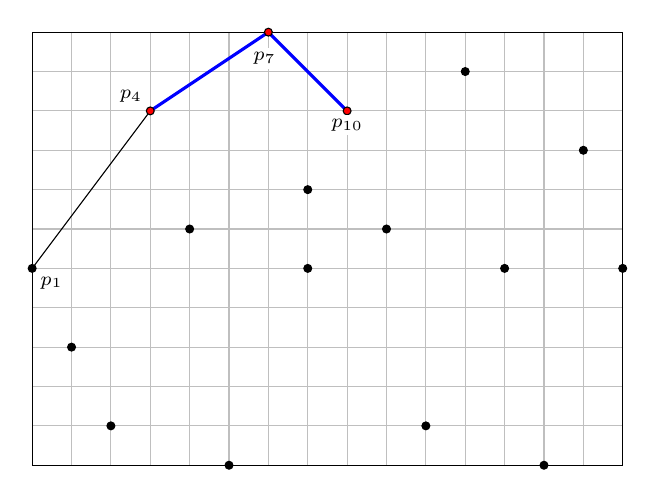
\begin{tikzpicture}[baseline=0]
            \tiktop
            
            \draw[black]
                (p1) -- (p4);
            \draw[blue, line width=0.4mm]
                (p4) -- (p7) -- (p10);

            \foreach \point/\a/\b/\i/\align/\co in {
                p1/7/0/1/above right/black,
                p2/8/3/2/above right/black,
                p3/4/9/3/above/black,
                p4/1/6/4/above/red,
                p5/2/2/5/above/black,
                p6/5/0/6/above/black,
                p7/6/11/7/below/red,
                p8/7/5/8/above/black,
                p9/7/7/9/above/black,
                p10/8/9/10/above/red,
                p11/9/6/11/above/black,
                p12/10/1/12/above/black,
                p13/11/10/13/below/black,
                p14/12/5/14/above/black,
                p15/13/0/15/above/black,
                p16/14/8/16/below left/black,
                p17/15/5/17/below left/black}{

                \draw[black,fill=\co]
                    let \p1 = (\point)
                    in (\x1, \y1) circle (0.5mm);
            }
            \foreach \point/\a/\b/\i/\align/\co in {
                p1/7/0/1/below right/black,
                p4/1/6/4/above left/black,
                p10/8/9/10/below/red}{

                \path
                    let \p1 = (\point)
                    in
                        node[\align, fill=white, inner sep=1.5, outer sep=1.5] at (\x1, \y1) {$\scriptstyle p_{\i} $};
            }
            \foreach \point/\a/\b/\i/\align/\co in {
                p7/6/11/7/below/black}{

                \path
                    let \p1 = (\point)
                    in
                        node[\align, xshift=-0.5mm, yshift=-1.5mm, fill=white, inner sep=1.5, outer sep=1.5] at (\x1, \y1) {$\scriptstyle p_{\i} $};
            }
        \end{tikzpicture}} &
        \makecell[l]{$\!\begin{aligned}
            & \Lupper = \kq{p_1,p_4, p_7, p_{10}}
        \end{aligned}$} \\
        % --- LINE 16 --------------------------------------------------------
        \noindent\parbox[c][\pich]{\picb}{
        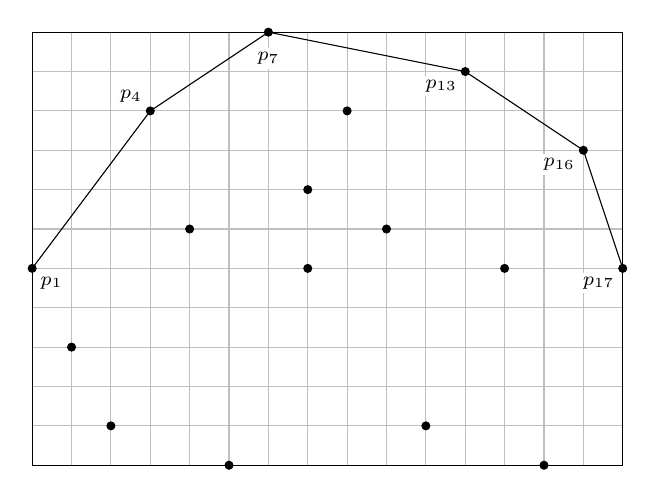
\begin{tikzpicture}[baseline=0]
            \tiktop
            
            \draw[black]
                (p1) -- (p4) -- (p7) -- (p13) -- (p16) -- (p17);

            \foreach \point/\a/\b/\i/\align/\co in {
                p1/7/0/1/above right/black,
                p2/8/3/2/above right/black,
                p3/4/9/3/above/black,
                p4/1/6/4/above/black,
                p5/2/2/5/above/black,
                p6/5/0/6/above/black,
                p7/6/11/7/below/black,
                p8/7/5/8/above/black,
                p9/7/7/9/above/black,
                p10/8/9/10/above/black,
                p11/9/6/11/above/black,
                p12/10/1/12/above/black,
                p13/11/10/13/below/black,
                p14/12/5/14/above/black,
                p15/13/0/15/above/black,
                p16/14/8/16/below left/black,
                p17/15/5/17/below left/black}{

                \draw[black,fill=\co]
                    let \p1 = (\point)
                    in (\x1, \y1) circle (0.5mm);
            }
            \foreach \point/\a/\b/\i/\align/\co in {
                p1/7/0/1/below right/black,
                p4/1/6/4/above left/black,
                p13/11/10/13/below left/black,
                p16/14/8/16/below left/black,
                p17/15/5/17/below left/black}{

                \path
                    let \p1 = (\point)
                    in
                        node[\align, fill=white, inner sep=1.5, outer sep=1.5] at (\x1, \y1) {$\scriptstyle p_{\i} $};
            }
            \foreach \point/\a/\b/\i/\align/\co in {
                p7/6/11/7/below/black}{

                \path
                    let \p1 = (\point)
                    in
                        node[\align, yshift=-1.5mm, fill=white, inner sep=1.5, outer sep=1.5] at (\x1, \y1) {$\scriptstyle p_{\i} $};
            }
        \end{tikzpicture}} &
        \makecell[l]{$\!\begin{aligned}
            & \Lupper = \kq{p_1,p_4, p_7, p_10}
        \end{aligned}$}
   \end{tabularx}
\end{document}